\documentclass{article}
\usepackage{tikz}
\usetikzlibrary{calc}

\begin{document}

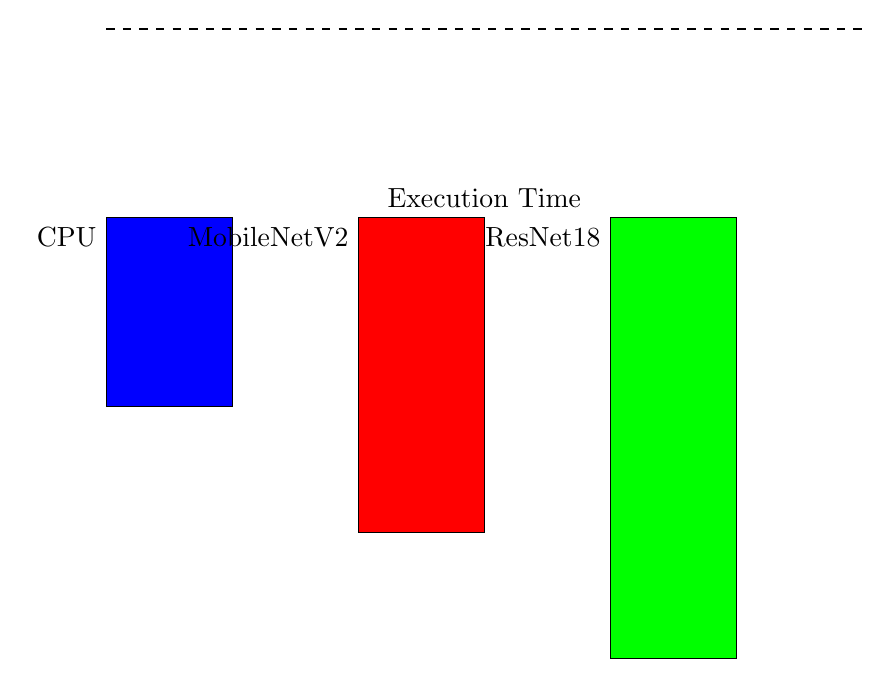
\begin{tikzpicture}[scale=0.8]
    % Define the coordinates
    \coordinate (A) at (0,0);
    \coordinate (B) at (4,0);
    \coordinate (C) at (8,0);
    \coordinate (D) at (12,0);
    
    % Draw the bars
    \draw[fill=blue] (A) rectangle ++(2,-3); % CPU
    \draw[fill=red] (B) rectangle ++(2,-5);  % MobileNetV2
    \draw[fill=green] (C) rectangle ++(2,-7); % ResNet18
    
    % Draw the line graph above the bars
    \draw[dashed, thick] ($(A)+(0,3)$) -- ($(D)+(0,3)$);
    \node at ($(A)!0.5!(D)$) [above] {Execution Time};
    
    % Add labels
    \node at (A) [below left] {CPU};
    \node at (B) [below left] {MobileNetV2};
    \node at (C) [below left] {ResNet18};
    
    % Eliminate the blue dot at the (0,0) coordinate
    \pgfset{
        /pgf/bar width=0pt,
        /pgf/plot style/.append style={bar width=0pt},
    }
\end{tikzpicture}

\end{document}